\documentclass[12pt, handout]{beamer}
\usepackage[polytechnique, psc, complexe, unicouleur]{persobeamer}
%nocouleur ou: unicouleur ou~: bicouleur
%complexe ou~: simple
%voir dans le package pour changer les couleurs
\usepackage{tikz}

\title{Projet Scientifique collectif INF02}
\subtitle{Soutenance finale}
\author{}
\date{19 mai 2015}


\begin{document}

  \addtobeamertemplate{frametitle}{}{%
    \begin{tikzpicture}[remember picture,overlay]
    \node[anchor=south east,yshift=2pt] at (current page.south east) {
\includegraphics[height=0.7cm]{logohori.eps}};

    \end{tikzpicture}
   }

    \begin{frame}
      \maketitle
    \end{frame}		


    %% sommaire %%		
    \begin{frame}
      \frametitle{Sommaire}
      %\tableofcontents[pausesections]
      \tableofcontents
    \end{frame}

%%%%%%%%%%%%%%%%%%%%%%%%
\section{Introduction}
%%%%%%%%%%%%%%%%%%%%%%%%%%

%%%%%%%%%%%%%%%%
\begin{frame}
 \frametitle{But du projet}
 Notre but était de produire un programme qui, étant donné un article sportif (de foot), serait capable d'en donner l'idée principale.
 
 La complexité de l'analyse syntaxique nous a amené à travailler sur des données pré-traitées contenant déjà l'information grammaticale du texte.

\end{frame}

%%%%%%%%%%%%%%%%%%%
\begin{frame}
 \frametitle{Modules}
 Nous avons pu séparer le travail en plusieurs modules relativement indépendants~:
 \begin{itemize}
  \item Construction d'un Réseau de Concepts contenant une information statique sur le monde~;
  \item Traitement des données grammaticales fournies par Systran~;
  \item Construction d'un Workspace représentant l'état de compréhension du texte~;
  \item Algorithme de résumé statistique servant de base de comparaison~;
  \item Algorithme de résumé abstractif utilisant ces divers modules.
 \end{itemize}
 
\end{frame}


\begin{frame}
 \frametitle{Outils extérieurs et points techniques}
 %% Je serais d'avis d'éliminer cette slide (Antonin)
 
\end{frame}

%%je pense qu'on peut franchement réduire l'état de l'art,
%% à un bref rappel.
%ce n'est pas ce qu'ils veulent entendre à une soutenance

\subsection{État de l'art}

\begin{frame}
 \frametitle{Traitement du langage naturel}
 Des outils existent déjà pour~:
 \begin{itemize}
  \item Reconnaître des mots, synonymes, etc. (nltk, wordnet)
  \item Établir la structure grammaticale d'une phrase (nltk, Systran)
 \end{itemize}
 Nous voulions utiliser ces outils pour résumer des textes.
 
\end{frame}

\begin{frame}
 \frametitle{\textit{Extractive summarization}}
 Un algorithme de résumé extractif~:
 \begin{itemize}
  \item Sépare les phrases du texte~;
  \item Note ces phrases d'après une étude statistique~;
  \item Sélectionne les phrases les mieux notées et les copie dans le résumé.
 \end{itemize}
 
\end{frame}

\begin{frame}
 \frametitle{\textit{Abstractive summarization}}
 Un algorithme de résumé abstractif tentera d'étudier les informations du texte~:
 \begin{itemize}
  \item Représentation du texte en mémoire sous forme d'un arbre syntaxique~;
  \item Élagage de cet arbre pour ne garder que les nœuds importants~;
  \item Génération d'un texte en langage naturel à partir de l'arbre simplifié.
 \end{itemize}
 On remarque que la première et la dernière étape sont beaucoup plus difficiles que leurs analogues en résumé extractif.
\end{frame}


\begin{frame}
 \frametitle{Génération du résumé et évaluation}
 %% D'avis de virer ça (Antonin)
 
\end{frame}

%je vire copycat/bascet, on détaillera mieux
%%sur le RC lui-même

\section{Sources de données}

%\subsection{Données textuelles}

\begin{frame}
 \frametitle{Données textuelles}
 \begin{itemize}
  \item Sélection d'un certain nombre de flux RSS pour téléchargement automatique d'articles~;
  \item Pré-traitement par une API (readability) pour n'obtenir que le corps de l'article.
 \end{itemize}
 
\end{frame}

%\subsection{Données conceptuelles}

\begin{frame}
 \frametitle{Extraction de concepts}
 
 
\end{frame}

\begin{frame}
 \frametitle{WordNet}
 
 
\end{frame}

\begin{frame}
 \frametitle{Conceptnet5}
 
 
\end{frame}

\begin{frame}
 \frametitle{Freebase}
 
 
\end{frame}


%%%%%%%%%%%%%%%%%%%%%%%%%%%
\section{Réseau de concepts}
%%%%%%%%%%%%%%%%%%%%%%%%%%%
% Schrotty !

\subsection{Structure}

\begin{frame}
 \frametitle{Objectifs et utilité du réseau}
 
 \begin{itemize}
  \item Représenter des données conceptuelles~;
  \item Établir des relations sémantiques~;
  \item Fournir des informations de contexte.
 \end{itemize}
 
 Le réseau n'effectue pas la \textbf{sélection} de l'information, mais il en ajoute.
 
\end{frame}


\begin{frame}[allowframebreaks = 0.7, fragile]
 \frametitle{Structure statique du réseau}
 
 \begin{block}{N\oe{}uds}
\begin{itemize}
 \item Étiquette~: concept~;
 \item Importance conceptuelle~;
 \item Activation~;
\end{itemize}

\textbf{Exemple~:} [``hyperactivity'', ``ic'': 34, ``a'': 10].

\end{block}
 
\begin{block}{Arêtes}
 \begin{itemize}
  \item Orientées~;
  \item Proximité~;
  \item Relation.
 \end{itemize}

\textbf{Exemple~:} [``hyperactivity'', ``disorder'', \{``r'': ``IsA'', ``w'': 47\}].
 
\end{block}

 
\end{frame}

%%%%%%%%%%%%%%%%%%%%%%%%%%%%%%%%%%%%%%%
\begin{frame}[fragile]
 \frametitle{Propriétés dynamiques du réseau}
 
 \begin{itemize}
  \item  L'activation d'un n\oe{}ud se propage à ses fils~;
  \item Les n\oe{}uds se désactivent naturellement.
 \end{itemize}
 
 \textbf{Exemple 1~:} en partant de \verb|``wayne_rooney''| et  \verb|``manchester_united_f.c.''|.
 
 \textbf{Exemple 2~:} en considérant les n\oe{}uds fortement activés (plus de 10\%).
 
 \note{Sur ce premier exemple, on ne montre pas le degré d'activation de chaque noeud, c'est juste pour voir la propagation. Sur le deuxième on s'intéresse déjà plus à la pertinence.}
 
\end{frame}


%%%%%%%%%%%%%%%%%%%%%%%%%%%%%%%
\begin{frame}
  \frametitle{Exemple 1}
% 
%    \begin{overprint}
% \onslide<1> Étape 0~: 2    n\oe{}uds activés.
% \onslide<2> Étape 1~: 6   n\oe{}uds activés.
% \onslide<3> Étape 2~: 67   n\oe{}uds activés.
% \onslide<4> Étape 3~: 51   n\oe{}uds activés.
% \onslide<5> Étape 4~: 59   n\oe{}uds activés.
% \onslide<6> Étape 5~: 133   n\oe{}uds activés.
% \end{overprint}
%   
%   \begin{overlayarea}{8cm}{8cm}
%    \only<1>{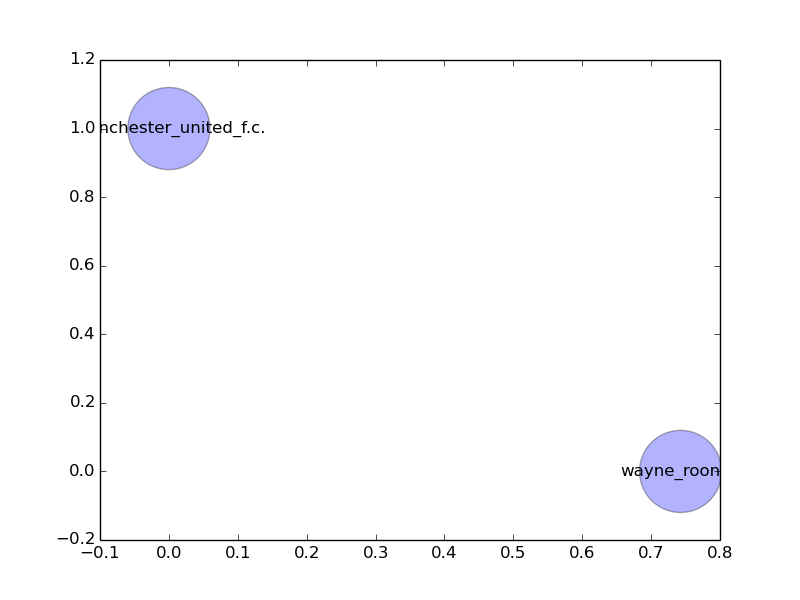
\includegraphics[height=7cm]{examples/touslesnoeuds/0.png}}
%    \only<2>{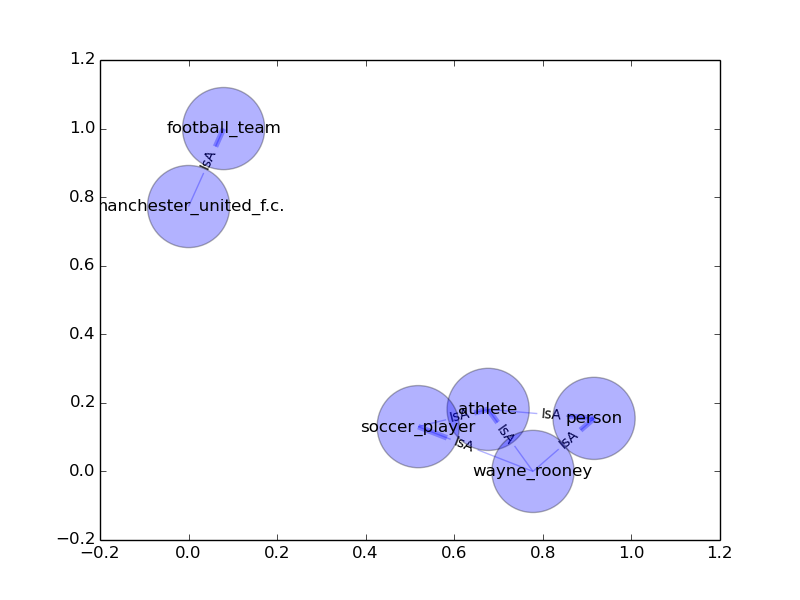
\includegraphics[height=7cm]{examples/touslesnoeuds/1.png}}
%    \only<3>{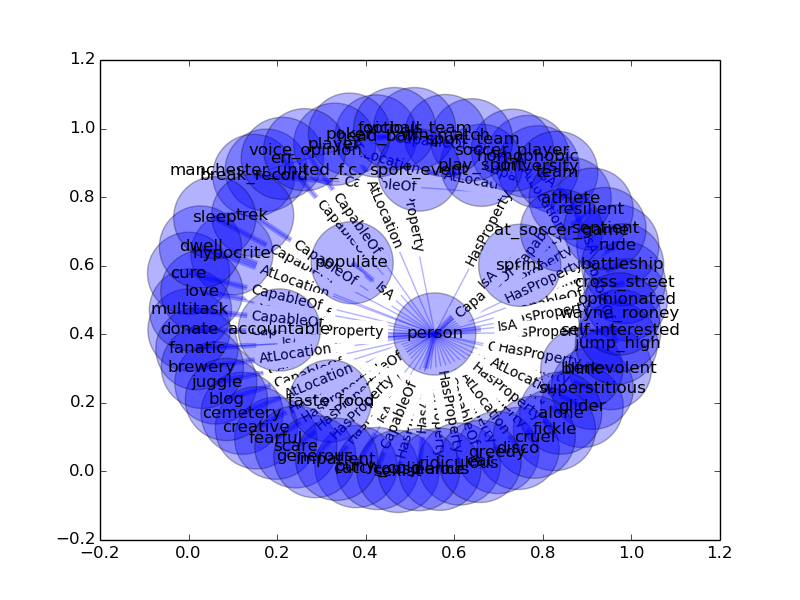
\includegraphics[height=7cm]{examples/touslesnoeuds/2.png}}
%    \only<4>{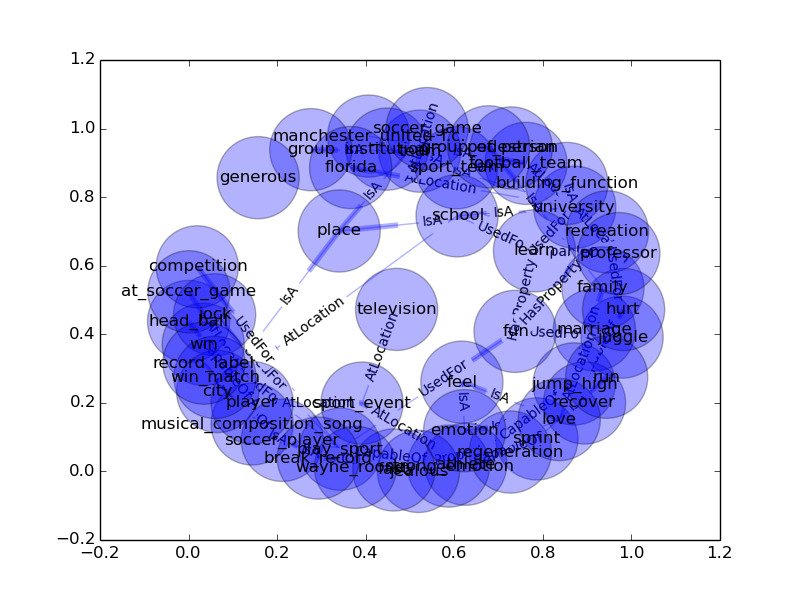
\includegraphics[height=7cm]{examples/touslesnoeuds/3.png}}
%    \only<5>{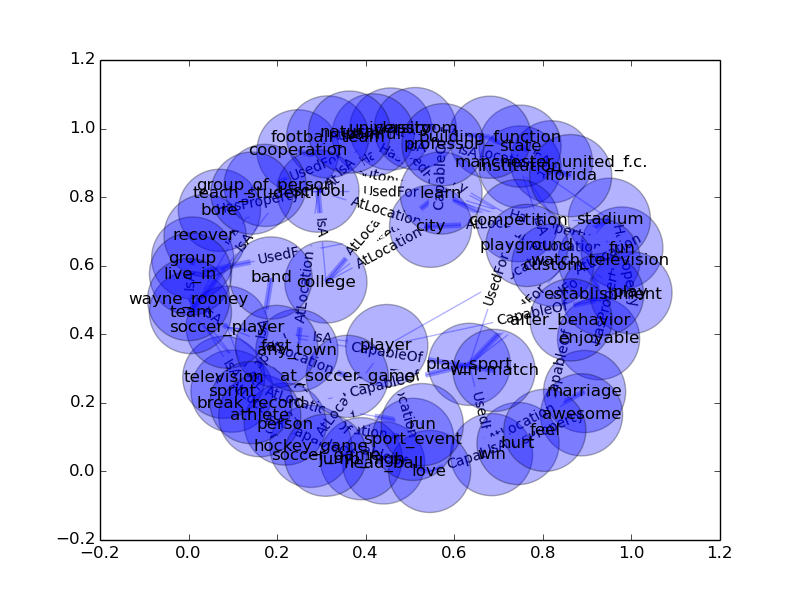
\includegraphics[height=7cm]{examples/touslesnoeuds/4.png}}
%    \only<6>{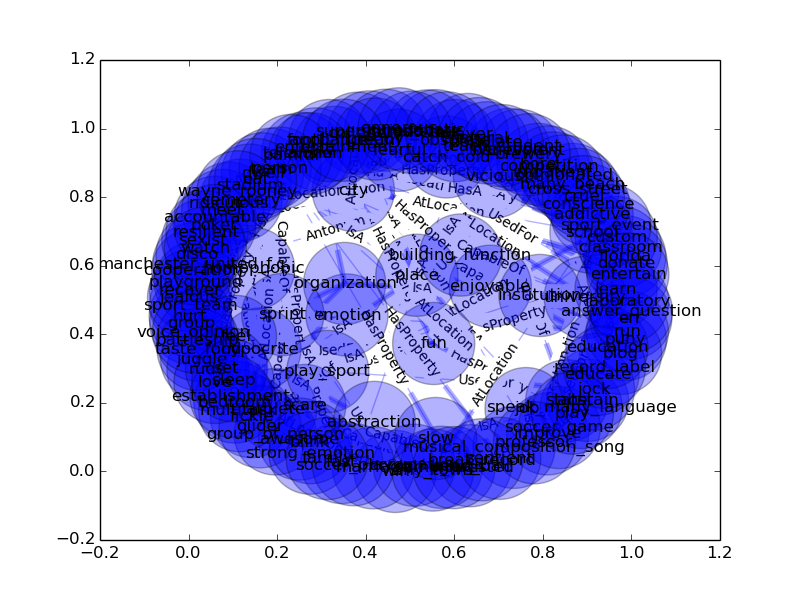
\includegraphics[height=7cm]{examples/touslesnoeuds/5.png}}
%    \only<7>{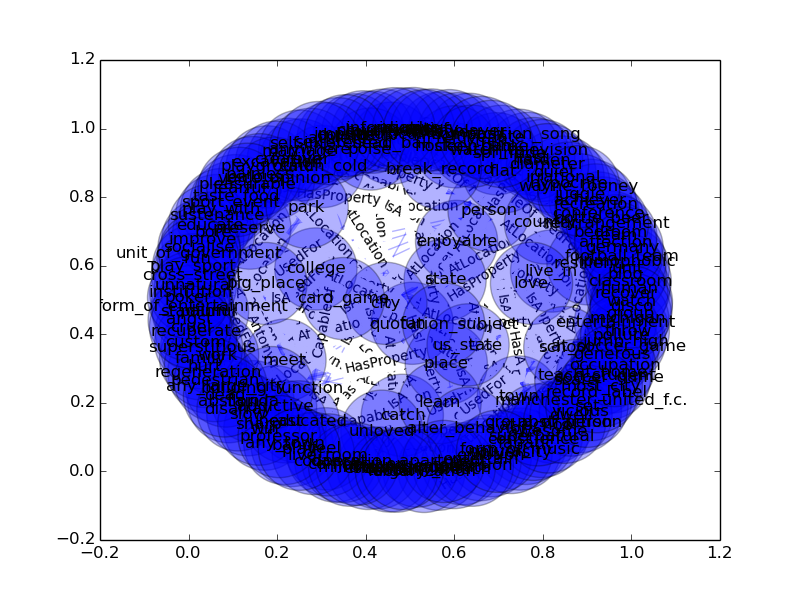
\includegraphics[height=7cm]{examples/touslesnoeuds/6.png}}
%   \end{overlayarea}

\end{frame}

%%%%%%%%%%%%%%%%%%%
\begin{frame}
  \frametitle{Exemple 2}
% 
%    \begin{overprint}
% \onslide<1> Étape 0~: 2    n\oe{}uds activés.
% \onslide<2> Étape 1~: 3    n\oe{}uds activés.
% \onslide<3> Étape 2~: 4    n\oe{}uds activés.
% \onslide<4> Étape 3~: 4   n\oe{}uds activés.
% \onslide<5> Étape 4~: 5   n\oe{}uds activés.
% \onslide<6> Étape 5~: 9   n\oe{}uds activés.
% \onslide<7> Étape 6~: 16   n\oe{}uds activés.
% \onslide<8> Étape 7~: 22   n\oe{}uds activés.
% \onslide<9> Étape 8~: 34   n\oe{}uds activés.
% \onslide<10> Étape 9~: 54   n\oe{}uds activés.
% \end{overprint}
% 
%   
%   \begin{overlayarea}{8cm}{8cm}
%    \only<1>{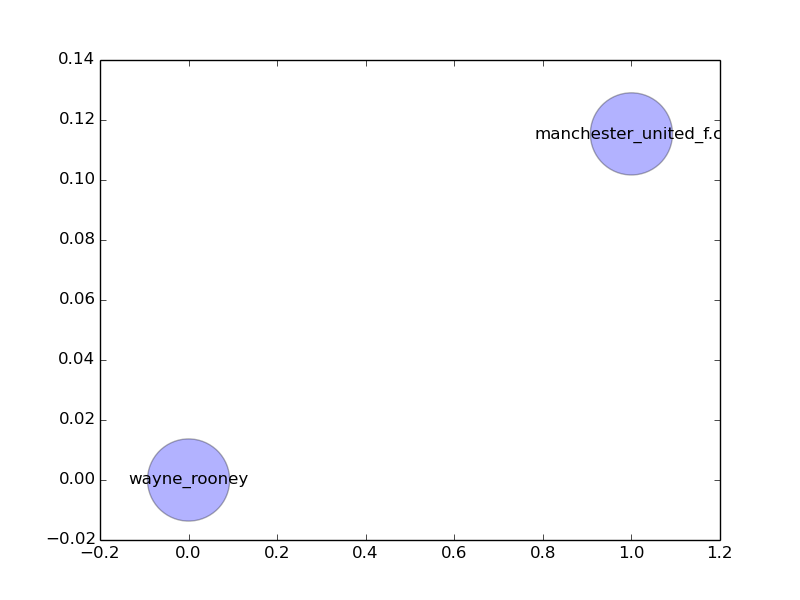
\includegraphics[height=7cm]{examples/noeudsbienactives/0.png}}
%    \only<2>{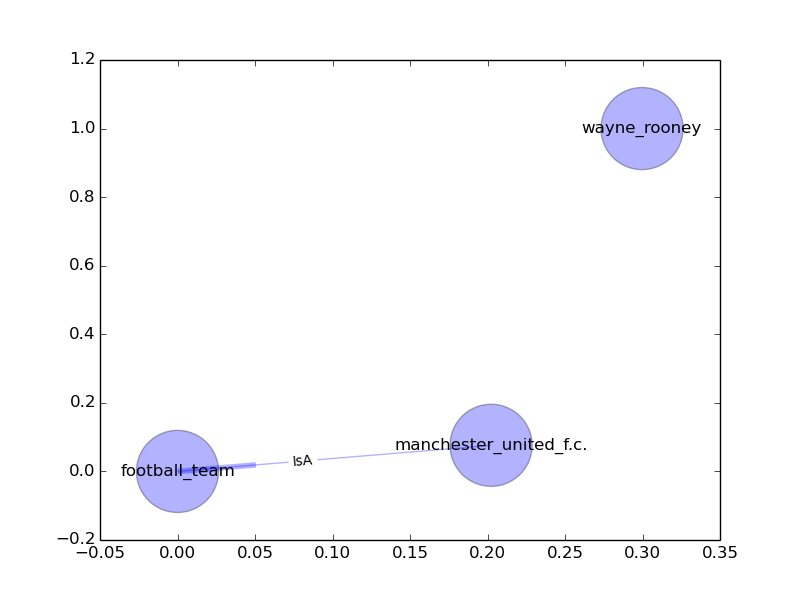
\includegraphics[height=7cm]{examples/noeudsbienactives/1.png}}
%    \only<3>{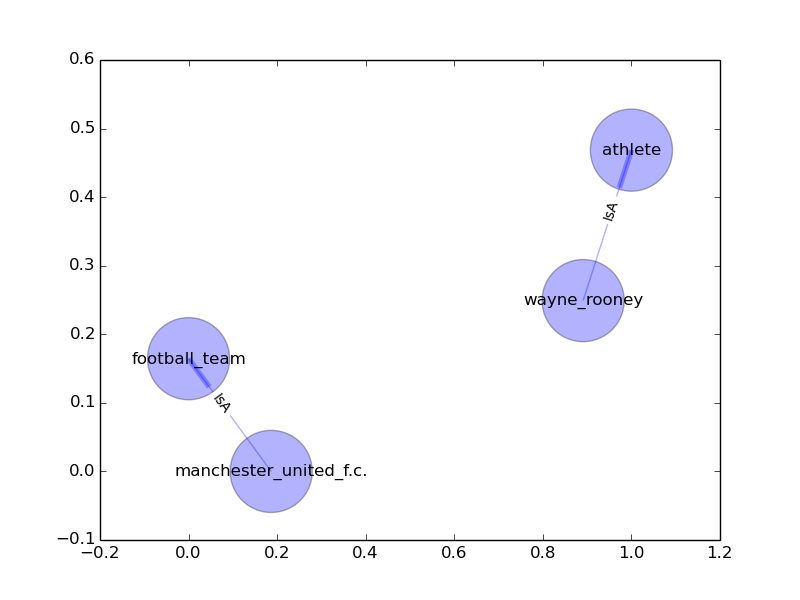
\includegraphics[height=7cm]{examples/noeudsbienactives/2.png}}
%    \only<4>{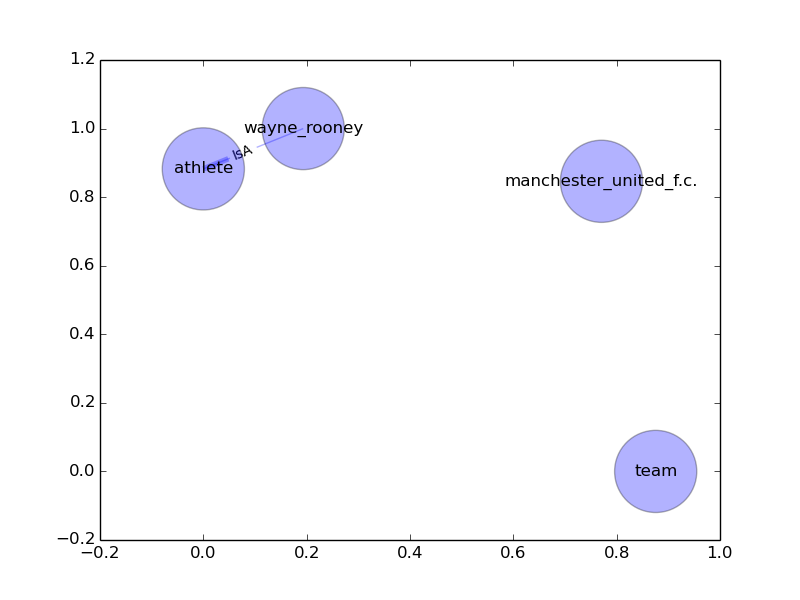
\includegraphics[height=7cm]{examples/noeudsbienactives/3.png}}
%    \only<5>{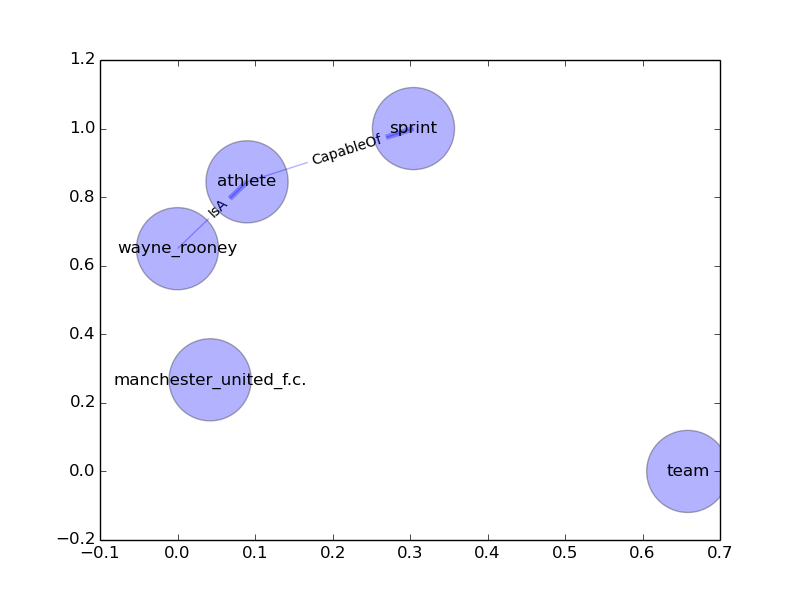
\includegraphics[height=7cm]{examples/noeudsbienactives/4.png}}
%    \only<6>{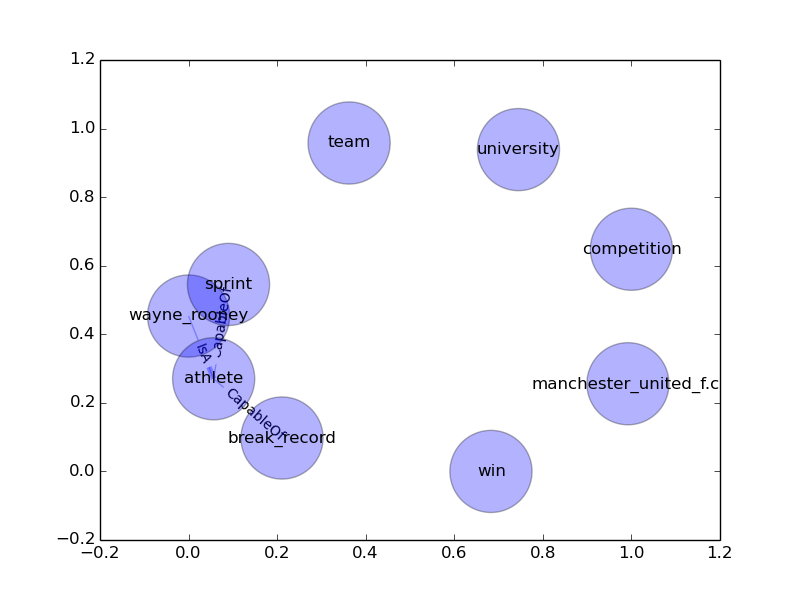
\includegraphics[height=7cm]{examples/noeudsbienactives/5.png}}
%    \only<7>{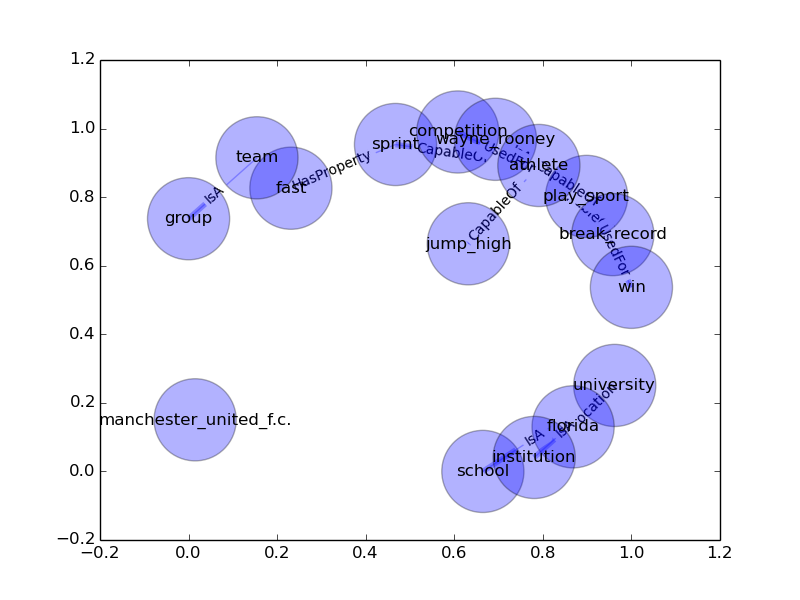
\includegraphics[height=7cm]{examples/noeudsbienactives/6.png}}
%    \only<8>{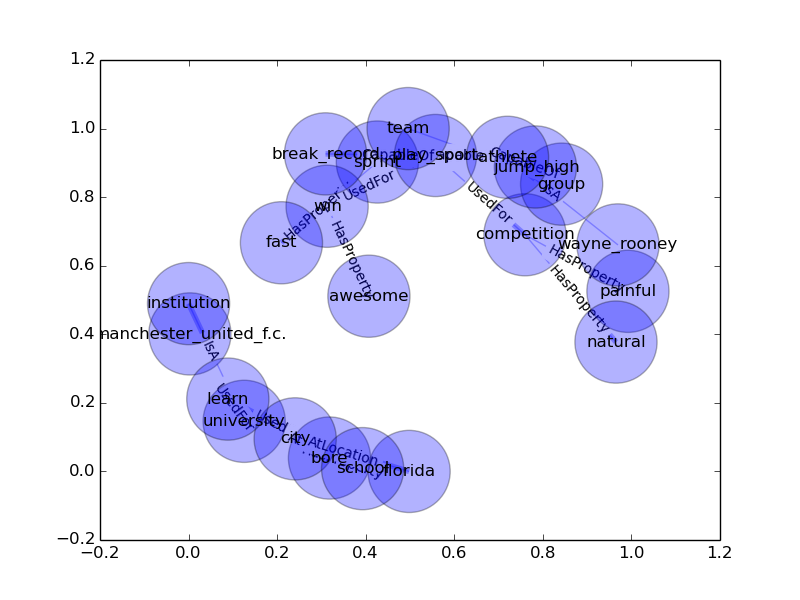
\includegraphics[height=7cm]{examples/noeudsbienactives/7.png}}
%    \only<9>{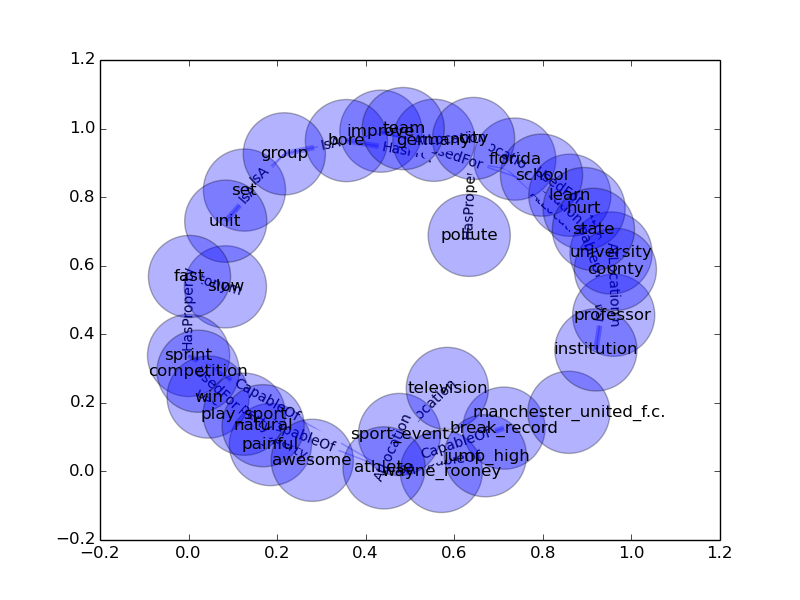
\includegraphics[height=7cm]{examples/noeudsbienactives/8.png}}
%    \only<10>{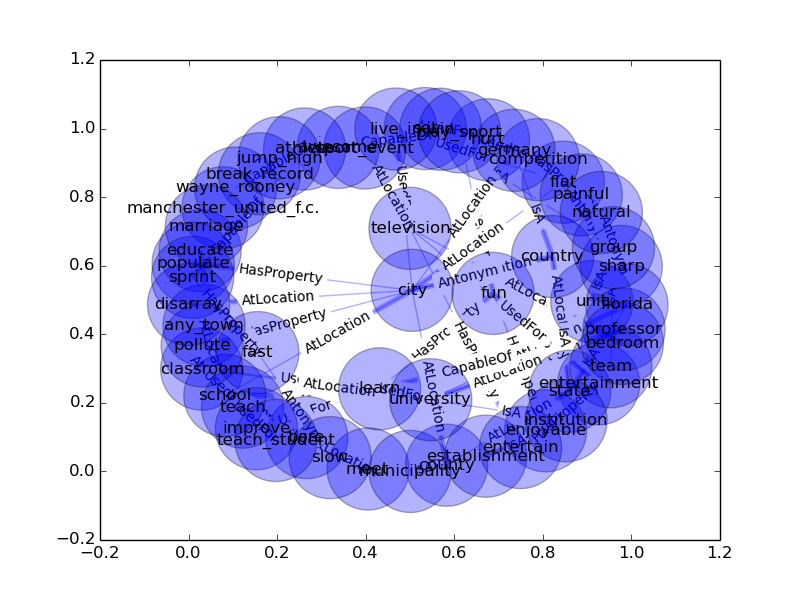
\includegraphics[height=7cm]{examples/noeudsbienactives/9.png}}
%   \end{overlayarea}

\end{frame}


%%%%%%%%%%%%%%%%%%%%%%%%%%%%%%%
\begin{frame}
 \frametitle{Détails}
 
 \begin{itemize}
  \item Les concepts ``font penser'' à d'autres concepts~: \textbf{contexte}~;
  \item Certains concepts sont oubliés~: \textbf{sélection}.
 \end{itemize}

 On ne cherche pas un état d'équilibre. Il faut tirer parti de ces deux propriétés en réglant le nombre d'étapes.
 
\end{frame}

\begin{frame}
  \frametitle{Désactivation}
 
 \begin{block}{Comment désactiver~?}
 \begin{itemize}
  \item En fonction de l'importance conceptuelle~;
  \item En fonction du nombre de liens.
  \end{itemize}
 \end{block}

 \textbf{Exemple 3~:}  N\oe{}uds bien activés, sans tenir compte du nombre de liens.
 
 \textbf{Exemple 4~:} En introduisant maintenant une dépendance du nombre de liens.
 
 \note{!!!! Pour l'importance conceptuelle, on verra plus tard avec les méthodes statistiques. Grosso modo, plus un noeud est important, moins vite il se désactive. Pour l'exemple 3, même exemple que le deuxième, mais avec cette fois un facteur log égal à 1, donc aucune dépendance avec le nombre de liens.}
 
 \note{Exemple pathologique~: un mot comme ``<water''> a 44 voisins avec de bons poids}
 
\end{frame}


%%%%%%%%%%%%%%%%%%%%%%%%%%%%%%%%%
\begin{frame}
\frametitle{Exemple 3}

%     \begin{overprint}
%       \onslide<1> Étape 0~: 2  n\oe{}uds activés.
%       \onslide<2> Étape 1~: 5  n\oe{}uds activés.
%       \onslide<3> Étape 2~: 14 n\oe{}uds activés.
%       \onslide<4> Étape 3~: 26 n\oe{}uds activés.
%       \onslide<5> Étape 4~: 51 n\oe{}uds activés.
%       \onslide<6> Étape 5~: 114 n\oe{}uds activés.
%       \onslide<7> Étape 6~: 209 n\oe{}uds activés.
%       \onslide<8> Étape 7~: 334 n\oe{}uds activés.
%     \end{overprint} 
% 
%   
%   \begin{overlayarea}{8cm}{8cm}
%    \only<1>{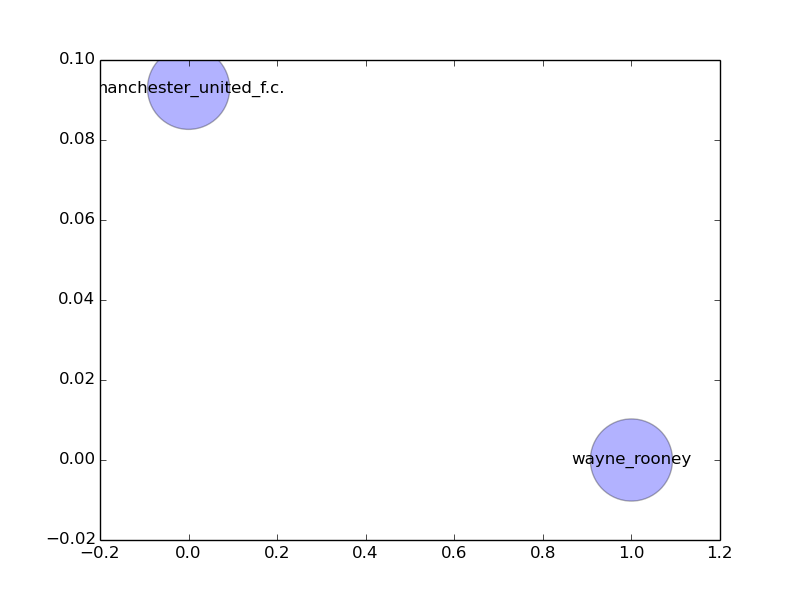
\includegraphics[height=7cm]{examples/facteurlogun/0.png}}
%    \only<2>{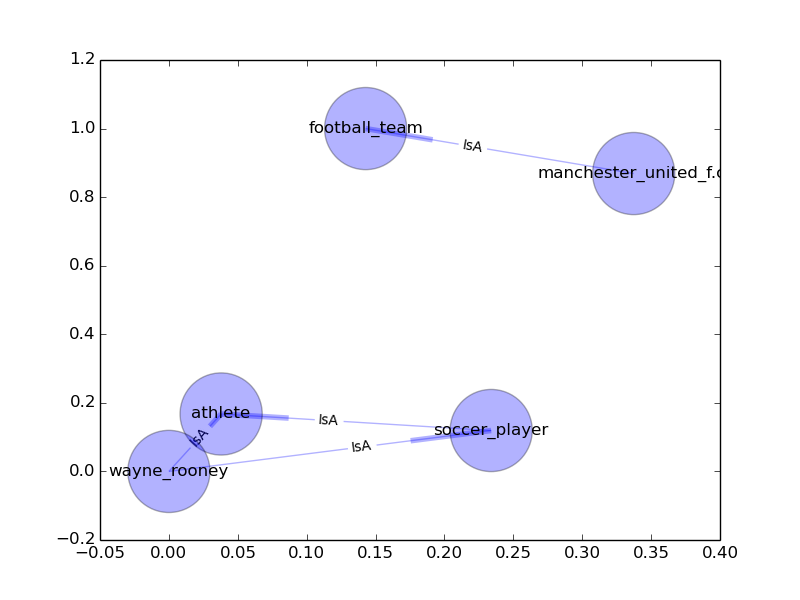
\includegraphics[height=7cm]{examples/facteurlogun/1.png}}
%    \only<3>{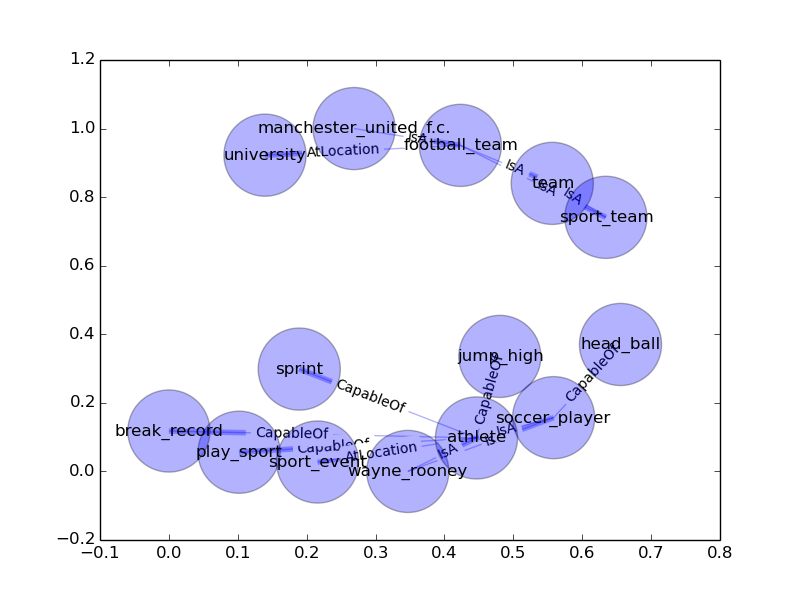
\includegraphics[height=7cm]{examples/facteurlogun/2.png}}
%    \only<4>{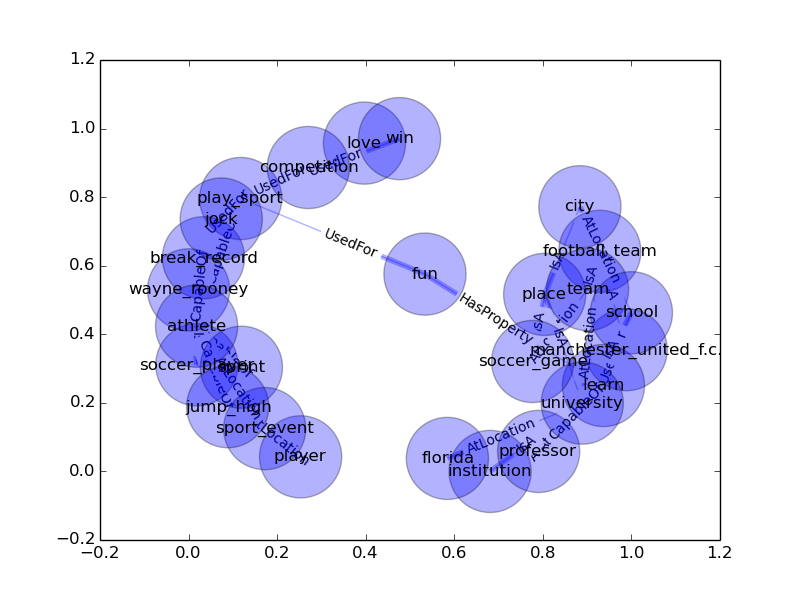
\includegraphics[height=7cm]{examples/facteurlogun/3.png}}
%    \only<5>{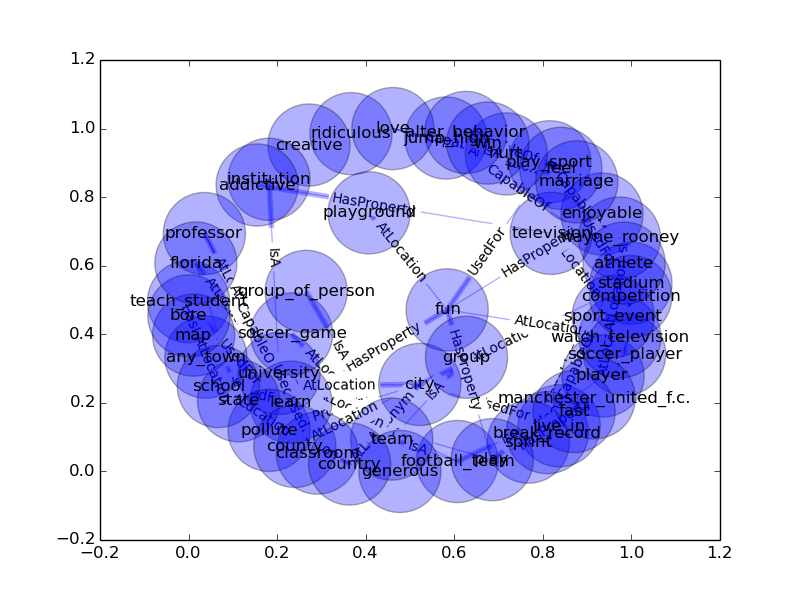
\includegraphics[height=7cm]{examples/facteurlogun/4.png}}
%    \only<6>{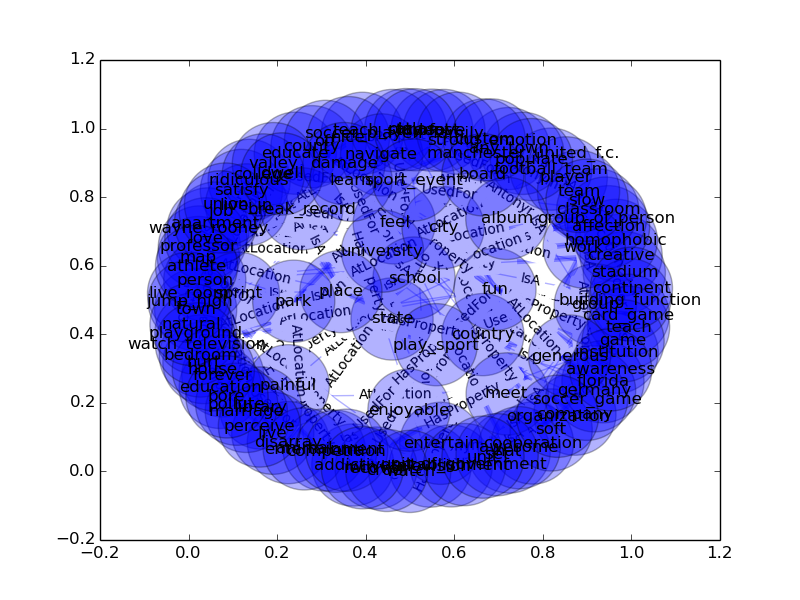
\includegraphics[height=7cm]{examples/facteurlogun/5.png}}
%    \only<7>{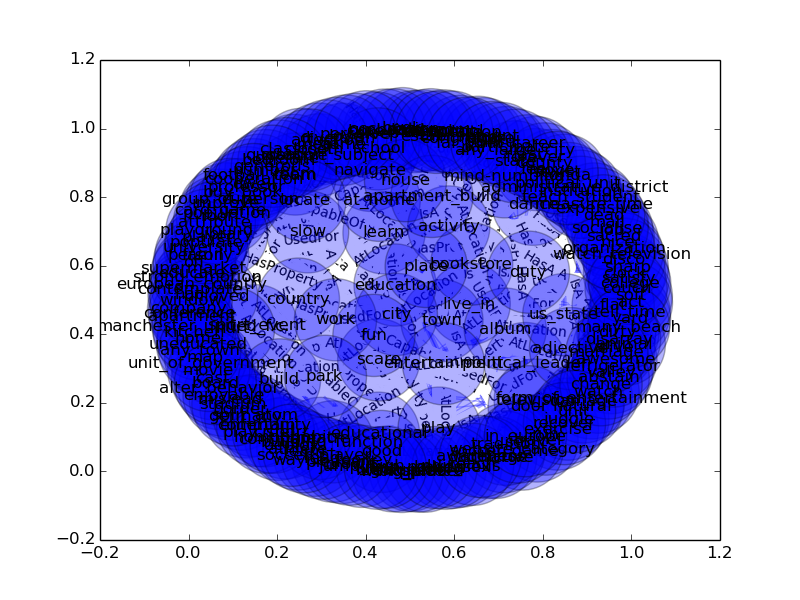
\includegraphics[height=7cm]{examples/facteurlogun/6.png}}
%    \only<8>{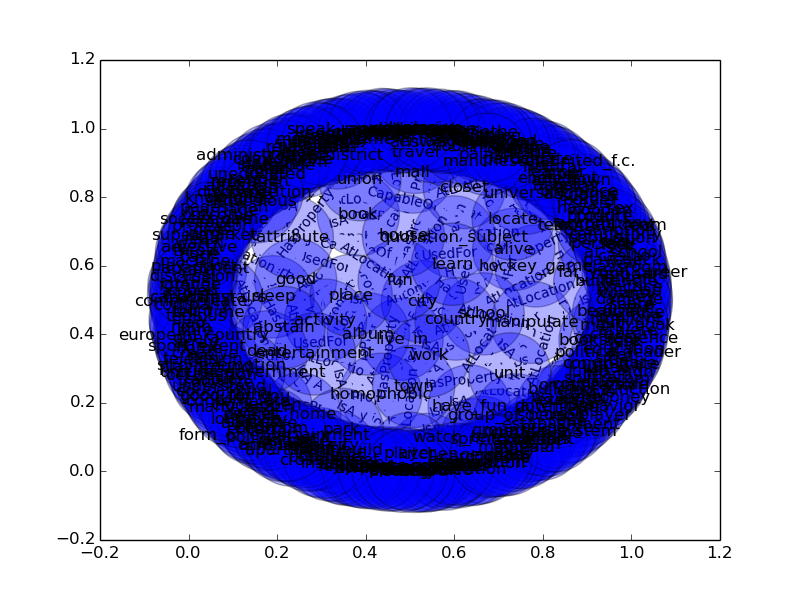
\includegraphics[height=7cm]{examples/facteurlogun/7.png}}
%   \end{overlayarea}

\end{frame}

%%%%%%%%%%%%%%%%%%%%%%%%%%%
\begin{frame}
 \frametitle{Exemple 4}
 
%     \begin{overprint}
%       \onslide<1> Étape 0~: 2  n\oe{}uds activés.
%       \onslide<2> Étape 1~: 3   n\oe{}uds activés.
%       \onslide<3> Étape 2~: 2  n\oe{}uds activés.
%       \onslide<4> Étape 3~: 3  n\oe{}uds activés.
%       \onslide<5> Étape 4~: 3  n\oe{}uds activés.
%       \onslide<6> Étape 5~: 4  n\oe{}uds activés.
%       \onslide<7> Étape 6~: 6  n\oe{}uds activés.
%       \onslide<8> Étape 7~: 9  n\oe{}uds activés.
%     \end{overprint} 
% 
%   
%   \begin{overlayarea}{8cm}{8cm}
%    \only<1>{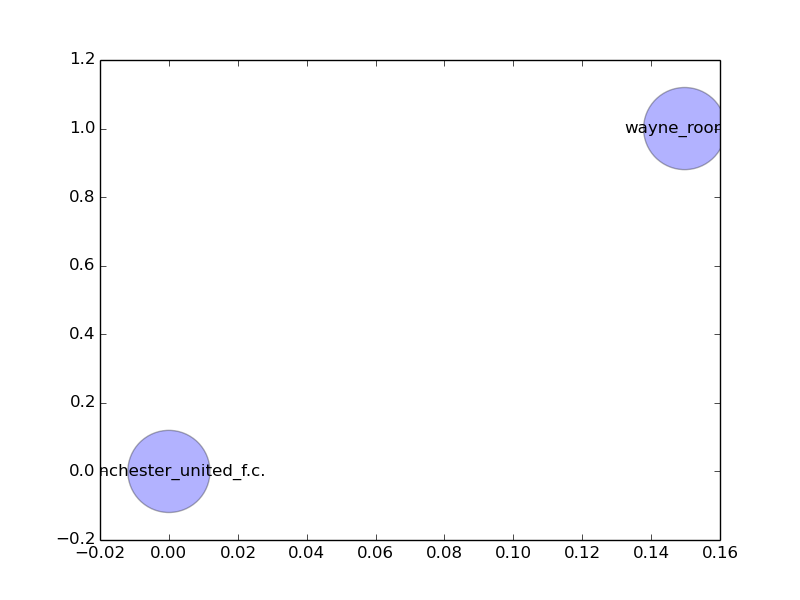
\includegraphics[height=7cm]{examples/grosfacteurlog/0.png}}
%    \only<2>{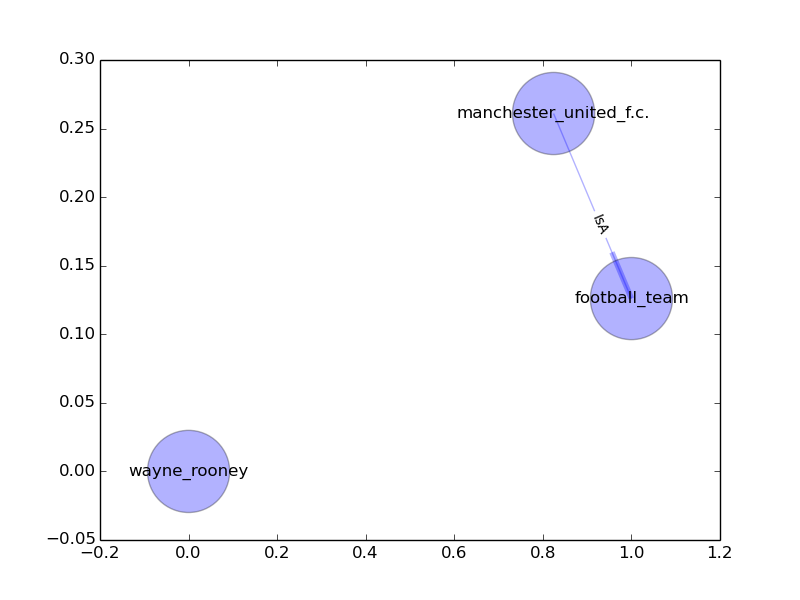
\includegraphics[height=7cm]{examples/grosfacteurlog/1.png}}
%    \only<3>{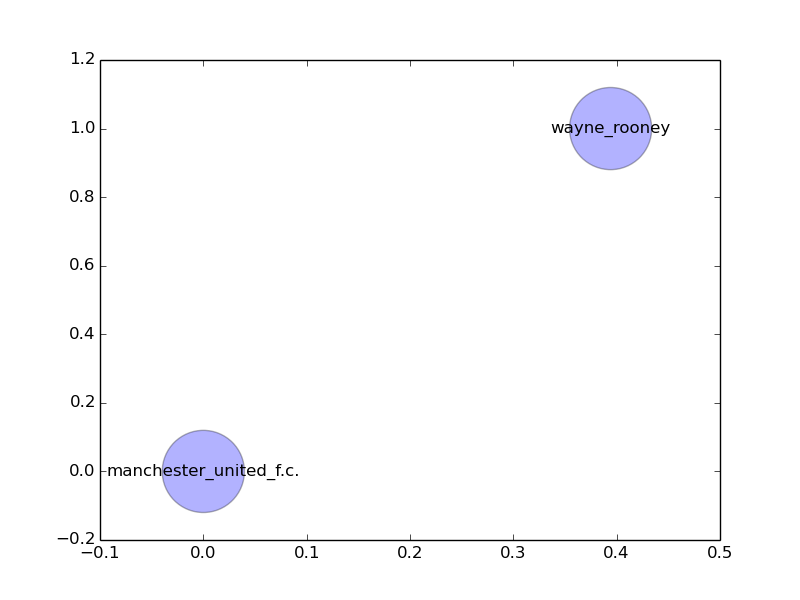
\includegraphics[height=7cm]{examples/grosfacteurlog/2.png}}
%    \only<4>{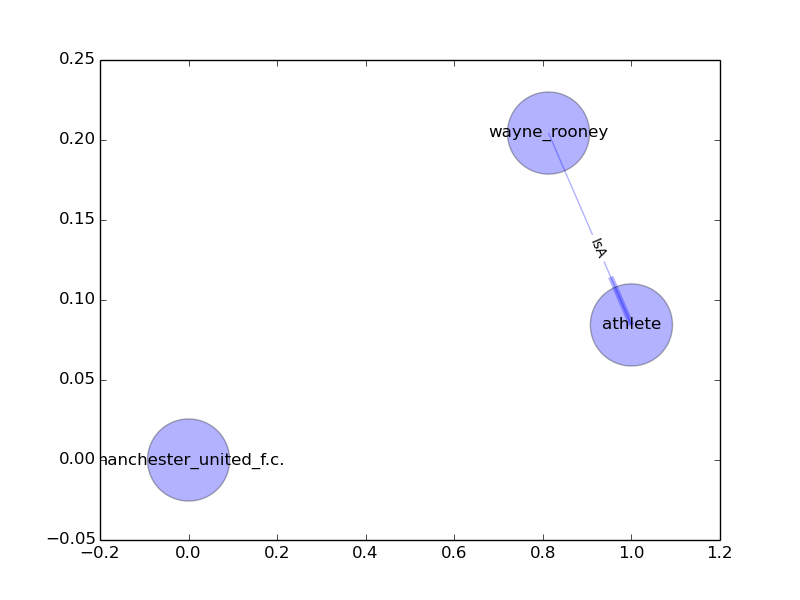
\includegraphics[height=7cm]{examples/grosfacteurlog/3.png}}
%    \only<5>{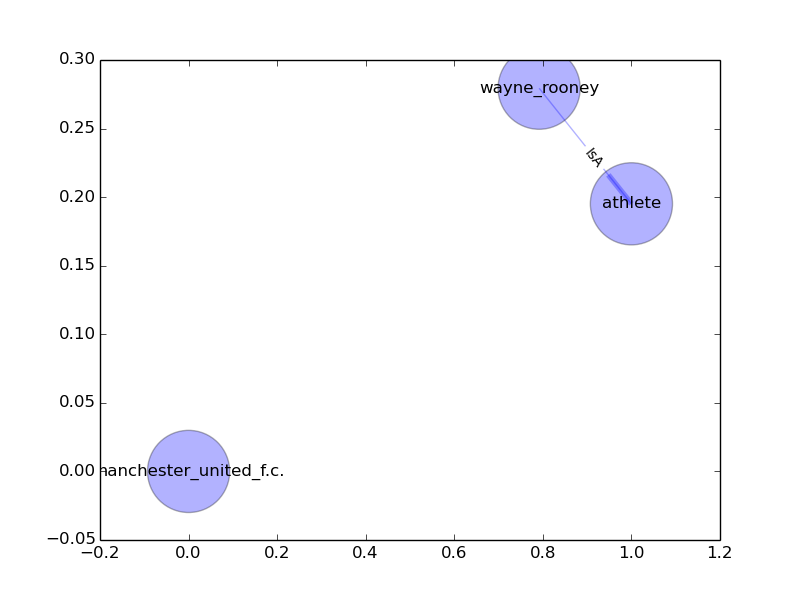
\includegraphics[height=7cm]{examples/grosfacteurlog/4.png}}
%    \only<6>{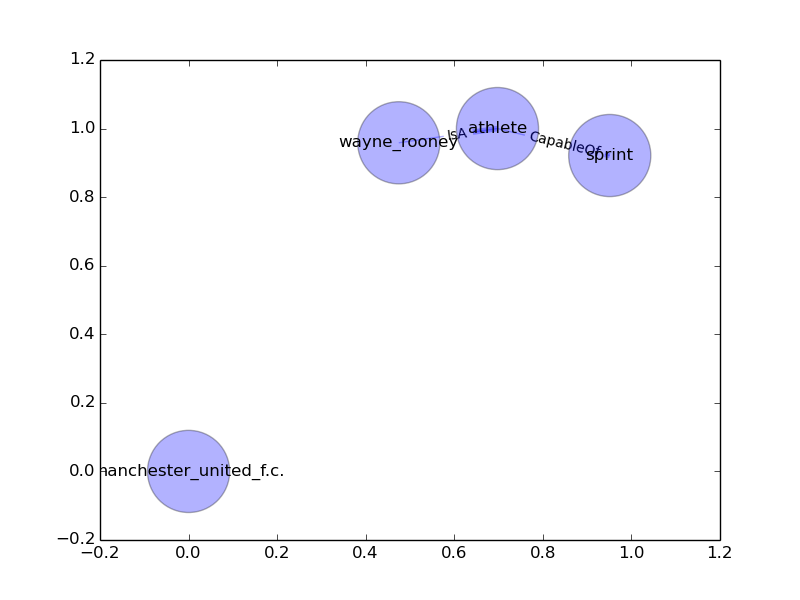
\includegraphics[height=7cm]{examples/grosfacteurlog/5.png}}
%    \only<7>{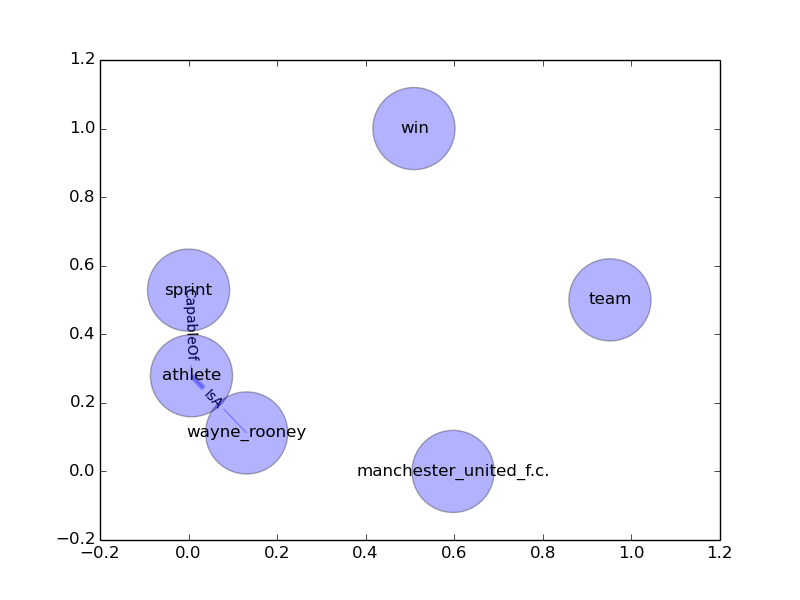
\includegraphics[height=7cm]{examples/grosfacteurlog/6.png}}
%    \only<8>{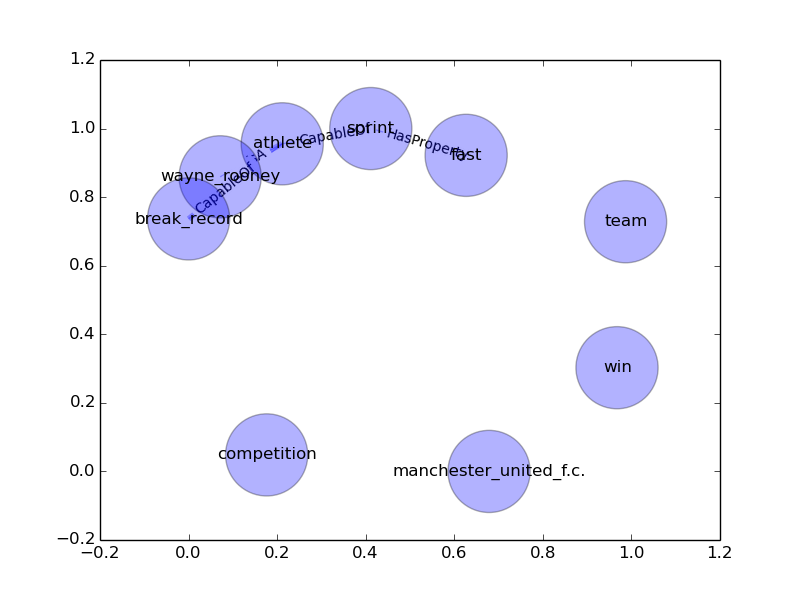
\includegraphics[height=7cm]{examples/grosfacteurlog/7.png}}
%   \end{overlayarea}

\end{frame}



%%%%%%%%%%%%%%%%%%%%%%%%%
\subsection{Construction}
%%%%%%%%%%%%%%%%%%%%%%%%

%%%%%%%%%%%%%%%%%%%%%%%%%%ù
\begin{frame}
 \frametitle{Construction du réseau}
 
 Récupération de listes~:
 
 \begin{itemize}
  \item De concepts (noms communs, verbes\ldots{})~;
  \item De noms propres.
 \end{itemize}

 \pause{}
 
 Lancement de requêtes~:
 \begin{itemize}
  \item Conceptnet5~;
  \item Freebase.
 \end{itemize}
 
 \pause{}
 
 Extension à partir des premiers n\oe{}uds, par d'autres requêtes.
 
 \note{Nous partons de texte brut, digéré avec différents outils.}
 
\end{frame}

%%%%%%%%%%%%%%
\begin{frame}
  \frametitle{Exemple obtenu}
  
  \begin{itemize}
   \item Plus de 18~000 noms propres et concepts comme base (ayant donné des résultats positifs lors des requêtes)~;
   \item Extension à plus de 28~000 n\oe{}uds bien reliés entre eux~;
   \item Plus de 16~000 n\oe{}uds sans lien entrant.
  \end{itemize}

\note{Les noeuds sans lien entrant ne seront pas activés si on ne les trouve pas tels quels dans un texte.}
  
\end{frame}

%%%%%%%%%%%%%%%%%%%%
\begin{frame}[fragile]
 \frametitle{Exemple obtenu}
 
 \begin{block}{Meilleurs en liens sortants}
  \begin{verbatim}
human~: 41
water~: 44
person~: 50
someone~: 161
something~: 192 
  \end{verbatim}
 \end{block}

  \begin{block}{Meilleurs en liens entrants}
    \begin{verbatim}
soccer_player~: 1931
soccer_midfielder~: 1575
athlete~: 2182
person~: 3469
organisation, country\ldots{}
    \end{verbatim}
  \end{block}
\end{frame}


%%optionnel, et même beaucoup trop chiant
\begin{frame}
 \frametitle{Choix de programmation}
 
 
\end{frame}



\section{TF-IDF et méthodes statistiques}


\begin{frame}
 \frametitle{Définition de l'indice TF-IDF}
 \begin{itemize}
  \item TF~: fréquence d'un terme~;
  \item IDF~: fréquence inverse de document~;
  \item TF-IDF et poids d'une phrase.
 \end{itemize}
 
\end{frame}

\begin{frame}
 \frametitle{TF-IDF pour résumer}
 \begin{itemize}
  \item Algorithme;
  	\begin{itemize}
  	\item Cacule de poids
  	\item Extraction de phrases
  	\end{itemize}
  \item Qualité de résumé.
 \end{itemize}
 
\end{frame}


\begin{frame}
 \frametitle{TF-IDF pour l'importance conceptuelle}
 \begin{itemize}
  	\item Qeulques charactères de l'importance conceptuelle
  	\item Le cacule adapté
  \end{itemize}
 
\end{frame}


\section{Traitement préalable des données}

%%\subsection{Analyse syntaxique}

\begin{frame}
 \frametitle{Grammaires}
 Une grammaire, c'est~:
 \begin{itemize}
  \item Un ensemble de feuilles de la forme (unité syntaxique) -> (liste de fonctions possibles)
  \item Un ensemble de règles pour découper la phrase en portions de plus en plus réduites.
 \end{itemize}
 La plupart des grammaires sont aujourd'hui stochastiques, et estiment quelle est la structure de phrase la plus probable.
 
\end{frame}

\begin{frame}
 \frametitle{État du texte en fin d'analyse}
 En fin d'analyse par l'algorithme de systran, le texte est une liste de mots contenant~:
 \begin{itemize}
  \item lui-même, tel que présent dans le texte~;
  \item la forme normale associée~;
  \item une liste de tags catégorisant le mot (humain, idée, etc.)~;
  \item une liste de liens étiquetés vers d'autres mots de la phrase.
 \end{itemize}
 
 Pour rendre ces données plus agréables à étudier, nous avons explicité la structure d'arbre ainsi créée dans une classe GrammarTree.
 
\end{frame}


\begin{frame}[allowframebreaks = 0.7]
 \frametitle{Résolution de pronoms}
 
 
\end{frame}


\section{Traitement du réseau}

\subsection{Workspace}

\begin{frame}
  \frametitle{Workspace}

  \begin{block}{Structure}
    \begin{itemize}
      \item «~Tableau noir~» contenant les structures en cours de construction
      \item «~Projection~» du texte dans un espace plus abstrait
    \end{itemize}
  \end{block}
  \begin{block}{Intérêt}
    \begin{itemize}
      \item Représente l'état de compréhension du texte
      \item À la fin du traitement, les structures importantes du workspace représentent l'information importante du texte
    \end{itemize}
  \end{block}

\end{frame}

\begin{frame}
  \frametitle{Workspace}
 
  \begin{block}{Construction}
    \begin{itemize}
      \item Construit comme un graphe à partir du texte précédemment analysé
      \item Modifié par confrontation avec le réseau de concepts
    \end{itemize}
  \end{block}
 
\end{frame}

\subsection{Algorithme final}

\begin{frame}
 \frametitle{Algorithme final}
 
 
\end{frame}

\begin{frame}
 \frametitle{Exemples}
 
 
\end{frame}

\section{Conclusion}

\begin{frame}
 \frametitle{Conclusion}
 
C'était vraiment trop mythe comme PSC\@.
 
\end{frame}

\end{document}
